\section{Methodology}
\label{sec:method}

In this section, we detail the architectural components of \method. The overarching framework is depicted in Figure~\ref{fig:pipeline}. \method operates in a purely training-free manner across the multi-stage diffusion process, combining attention-level orthogonal feature decomposition, temporal Sigmoid scheduling, score-orthogonal gradient guidance on the latent manifold, and clean-latent statistical pushforward.

\begin{figure*}[t]
\centering
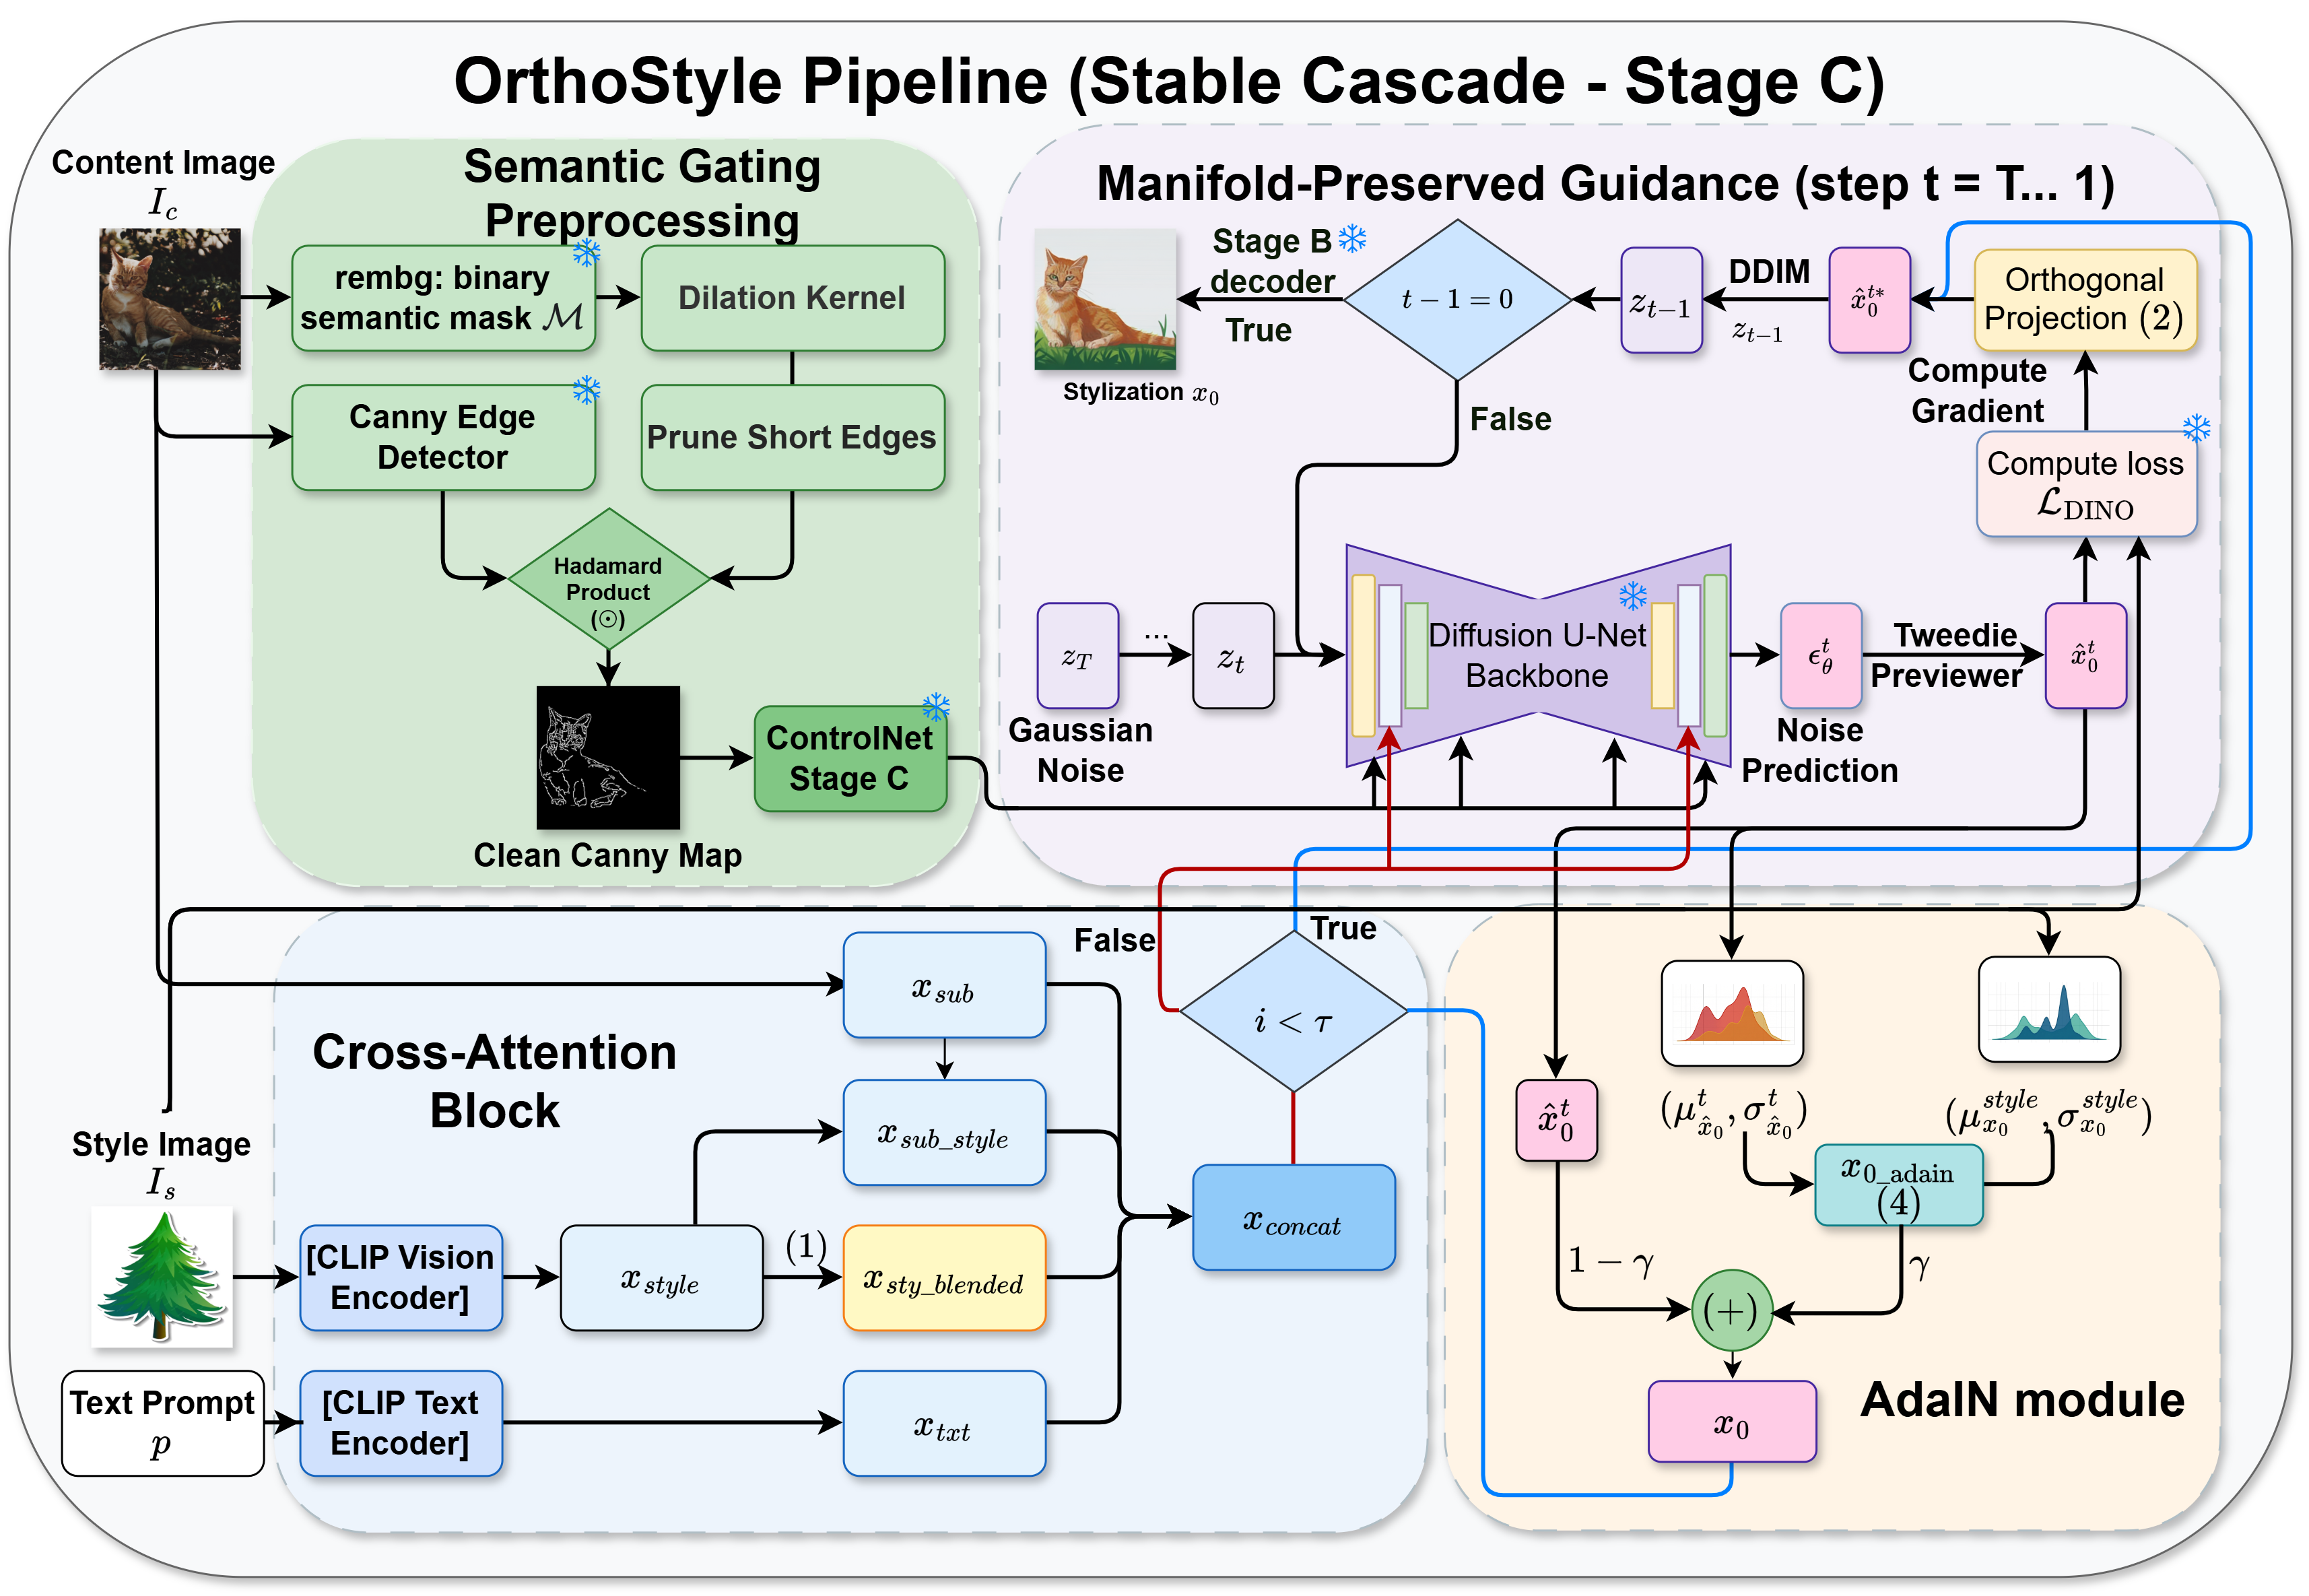
\includegraphics[width=\textwidth]{figs/pipeline.png}
\caption{\textbf{Comprehensive Pipeline of \method.} (Top) Cross-attention layers decouple content and style into orthogonal subspaces with energy compensation. (Bottom) During reverse diffusion, DINO-ViT terminal guidance computes score-orthogonal gradients to navigate the valid data manifold, assisted by early-stage clean latent AdaIN pushforward and semantic Canny structural gating.}
\label{fig:pipeline}
\end{figure*}

\subsection{Multi-Stream Cross-Attention Decomposition}
\label{subsec:attn_decomp}
Let $\bx \in \R^{B \times (H \cdot W) \times C}$ be the intermediate spatial query representations within an attention block of the generator, and $\mathbf{kv} \in \R^{B \times L \times C}$ denote the concatenated key-value tokens containing both text embeddings and visual CLIP prefix tokens of length $L_{\text{clip}}$.

Instead of computing a single entangled attention output, \method decomposes the conditioning stream into four distinct semantic components:
\begin{enumerate}
    \item \textbf{Text Stream} ($\xtxt$): Attends purely to text prompt tokens $\mathbf{kv}_{:\,-2L_{\text{clip}}}$, ensuring conceptual prompt grounding.
    \item \textbf{Subject Stream} ($\xsub$): Attends to the reference content/subject tokens $\mathbf{kv}_{:\,-L_{\text{clip}}}$, encoding the geometric silhouette, pose, and spatial layout of the target object.
    \item \textbf{Style Stream} ($\xstyle$): Attends to pure style tokens with mean token blending:
    \begin{equation}
        \mathbf{t}_{\text{blended}} = \alpha_s \mathbf{t}_{\text{style}} + (1 - \alpha_s) \left( \frac{1}{L_{\text{clip}}} \sum_{j=1}^{L_{\text{clip}}} \mathbf{t}_{\text{style}}^{(j)} \right),
    \end{equation}
    where $\alpha_s = 0.85$, smoothing high-frequency semantic noise while retaining artistic texture signatures.
    \item \textbf{Subject-Style Composite Stream} ($\xsubstyle$): Attends to the joint concatenation of subject and blended style tokens.
\end{enumerate}

\subsection{Orthogonal Feature Projection with Energy Compensation}
\label{subsec:ortho_proj}
A primary driver of content leakage is the naive linear summation of $\xstyle$ and $\xsub$, where semantic features collinear with $\xsub$ (such as objects embedded in the style image) directly inject foreign content into the generated image.

To strictly eliminate this interference, \method projects $\xstyle$ and $\xsubstyle$ onto the orthogonal complement of the subject subspace $\Vortho = \{ \bv \mid \inner{\bv}{\xsub} = 0 \}$.

\paragraph{Mathematical Formulation.}
For each spatial location, we compute the squared norm of the subject feature:
\begin{equation}
    \norm{\xsub}_2^2 = \sum_{c=1}^C (\xsub^{(c)})^2 + \epsilon_{\text{safe}},
\end{equation}
where $\epsilon_{\text{safe}} = 10^{-8}$. The parallel projection of the style representation onto the subject vector is:
\begin{equation}
    \Proj_{\xsub}(\xstyle) = \left( \frac{\inner{\xstyle}{\xsub}}{\norm{\xsub}_2^2} \right) \xsub.
\end{equation}
The orthogonalized style feature $\xstyleortho$ is then obtained via subspace subtraction:
\begin{equation}
    \xstyleortho = \xstyle - \Proj_{\xsub}(\xstyle).
    \label{eq:ortho_sub}
\end{equation}
By construction, $\inner{\xstyleortho}{\xsub} = 0$.

\paragraph{Energy Compensation (Norm Scaling).}
While Eq.~\eqref{eq:ortho_sub} removes collinear content leakage, orthogonal projection geometrically diminishes the feature magnitude: $\norm{\xstyleortho}_2 = \norm{\xstyle}_2 \sin \theta \le \norm{\xstyle}_2$. In severe cases, this leads to an under-stylized image where texture intensity is drastically muted.

To restore stylistic expressiveness without re-introducing content leakage, we introduce an exact \textit{Energy Compensation} operator:
\begin{equation}
    \tilde{\bx}_{\text{style}}^\perp = \xstyleortho \cdot \left( \frac{\norm{\xstyle}_2}{\norm{\xstyleortho}_2 + \epsilon_{\text{safe}}} \right).
    \label{eq:energy_comp}
\end{equation}
Applying the identical projection and energy compensation to $\xsubstyle$ yields $\tilde{\bx}_{\text{sub\_style}}^\perp$. 

The finalized attention feature $\bx_{\text{fused}}$ is synthesized via:
\begin{equation}
    \bx_{\text{fused}} = \wtxt \xtxt + \wsub \xsub + \wstyle \tilde{\bx}_{\text{style}}^\perp + \wsubstyle \tilde{\bx}_{\text{sub\_style}}^\perp.
    \label{eq:attn_synthesis}
\end{equation}

\subsection{Adaptive Feature Allocation (AFA) via Sigmoid Scheduling}
\label{subsec:afa}
The generation process undergoes distinct perceptual regimes: early timesteps establish coarse spatial layout and geometry, while later timesteps synthesize high-frequency textures. Fixed static weights fail to accommodate this dynamic.

We formulate an analytical temporal Sigmoid modulation function $S(p)$ over the normalized timestep progress $p = i / N_{\text{steps}} \in [0, 1]$:
\begin{equation}
    S(p) = \frac{1}{1 + \exp\left( -k (p - p_{\text{switch}}) \right)},
    \label{eq:sigmoid_schedule}
\end{equation}
where $p_{\text{switch}} = 0.10$ defines the critical transition inflection point, and $k = 50.0$ governs the transition steepness.

The time-varying attention weights are dynamically governed by:
\begin{align}
    \wtxt(p) &= 0.0, \\
    \wsub(p) &= 1.0 - 0.85 \cdot S(p), \\
    \wstyle(p) &= 0.45 \cdot S(p), \\
    \wsubstyle(p) &= 0.40 \cdot S(p).
\end{align}
During the first $10\%$ of sampling ($p \le p_{\text{switch}}$), $S(p) \approx 0 \implies \wsub \approx 1.0$, anchoring the rigid spatial geometry of the target content. As $p > p_{\text{switch}}$, $S(p) \to 1.0$, enabling aggressive, leakage-free style injection through the orthogonal channels.

\subsection{Score-Orthogonal DINO Latent Guidance}
\label{subsec:score_ortho}
To supervise style fidelity beyond attention modulation, we apply terminal cost guidance on the estimated clean latent $\bx_0$.

\paragraph{DINO-ViT Style Descriptor.}
Unlike CLIP (which overfits to categorical semantic labels) or CSD (which suffers from domain collapse on unseen artistic media), self-supervised Vision Transformers (DINO-ViT)~\cite{caron2021emerging} construct spatial self-attention features that naturally encode artistic brushstrokes, textures, and color distribution.

At each step $i < \tau$, we decode the predicted clean latent $\bz_0 = \bx_0$ to pixel space using a lightweight previewer network $\hat{I}_0 = \mathcal{P}(\bz_0)$ and compute the mean squared error in DINO feature space:
\begin{equation}
    \Loss_{\text{style}}(\bz_0) = \norm{ \rho\left( \text{pre}(\hat{I}_0) \right) - \rho\left( \text{pre}(I_{\text{style}}) \right) }_2^2,
\end{equation}
where $\rho(\cdot)$ denotes the feature extraction function of a pre-trained DINO-ViT-S/16 model.

\paragraph{Score-Orthogonal Projection on Data Manifold.}
Standard gradient guidance updates $\bz_0 \leftarrow \bz_0 - \eta \nabla_{\bz_0} \Loss_{\text{style}}$. However, the unconstrained gradient $\bg = \nabla_{\bz_0} (\lambda_{\text{style}} \Loss_{\text{style}})$ contains strong components parallel to the reverse diffusion score direction $\beps_\theta$, pushing latents off the valid manifold of realistic images.

We project the guidance gradient $\bg$ onto the subspace orthogonal to the predicted score vector $\beps_\theta$:
\begin{equation}
    \Proj_{\beps_\theta}(\bg) = \left( \frac{\inner{\bg}{\beps_\theta}}{\norm{\beps_\theta}_2^2 + \epsilon_{\text{safe}}} \right) \beps_\theta,
\end{equation}
\begin{equation}
    \bg^\perp = \bg - \Proj_{\beps_\theta}(\bg).
\end{equation}
The clean latent is updated along this safe tangent trajectory using a decaying step size:
\begin{equation}
    \bz_0 \leftarrow \bz_0 - \eta \left( 1 - \frac{i}{N_{\text{steps}}} \right) \bg^\perp.
    \label{eq:latent_update}
\end{equation}

\subsection{Clean Latent ($x_0$) AdaIN Pushforward}
\label{subsec:adain}
To rapidly align the global chromatic palette and contrast of the target subject with the style exemplar, we apply an Adaptive Instance Normalization (AdaIN)~\cite{huang2017arbitrary} pushforward directly on the predicted clean latent $\bx_0$ during the initial timesteps $i < \tau_{\text{pushforward}}$ ($\tau_{\text{pushforward}} = 5$):
\begin{equation}
    \bx_0^{\text{adain}} = \left( \frac{\bx_0 - \bmu(\bx_0)}{\bsigma(\bx_0) + \epsilon} \right) \odot \bsigma(\bx_0^{\text{style}}) + \bmu(\bx_0^{\text{style}}),
\end{equation}
\begin{equation}
    \bx_0 \leftarrow (1 - \gamma_{\text{push}}) \bx_0 + \gamma_{\text{push}} \bx_0^{\text{adain}},
\end{equation}
where $\gamma_{\text{push}} = 0.60$. Operating on clean latents $\bx_0$ rather than noisy latents $\bx_t$ locks the global color tone without disturbing the Wiener diffusion variance schedule.

\subsection{Semantic Canny Structural Gating}
\label{subsec:canny}
To enforce crisp subject contours while discarding distracting background clutter, we extract semantic masks $\mathcal{M} \in \{0, 1\}^{H \times W}$ using salient background removal (rembg). The raw Canny edge map $C_{\text{noisy}}$ is filtered via hard morphological gating:
\begin{equation}
    C_{\text{clean}} = C_{\text{noisy}} \odot \text{Dilation}(\mathcal{M}, \text{kernel}=5).
\end{equation}
The clean edge map is fed into a Stage C ControlNet with condition scaling $\lambda_{\text{cnet}} = 0.8$, guaranteeing flawless anatomical boundaries.
